\documentclass{beamer}
\usetheme[compress]{Ilmenau}
\usepackage{stmaryrd}
\usepackage{graphicx}
%\usepackage{animate}

\title{Real-Time Associative Classification Algorithms for High-Dimensional Streaming Data}
\author{Adriano Veloso}
\institute{DCC-UFMG}
\date{}

\begin{document}

\begin{frame}
\titlepage
\end{frame}

\section{Scenario}

\begin{frame}\frametitle{High-Dimensional Streaming Data}

We are experiencing a revolution in the capacity to quickly collect and transport large amounts of data.

\begin{itemize}
\item Data is produced and collected continuously
\item Data complexity and dimensionality is increasing
\end{itemize}

\begin{figure}
\centering
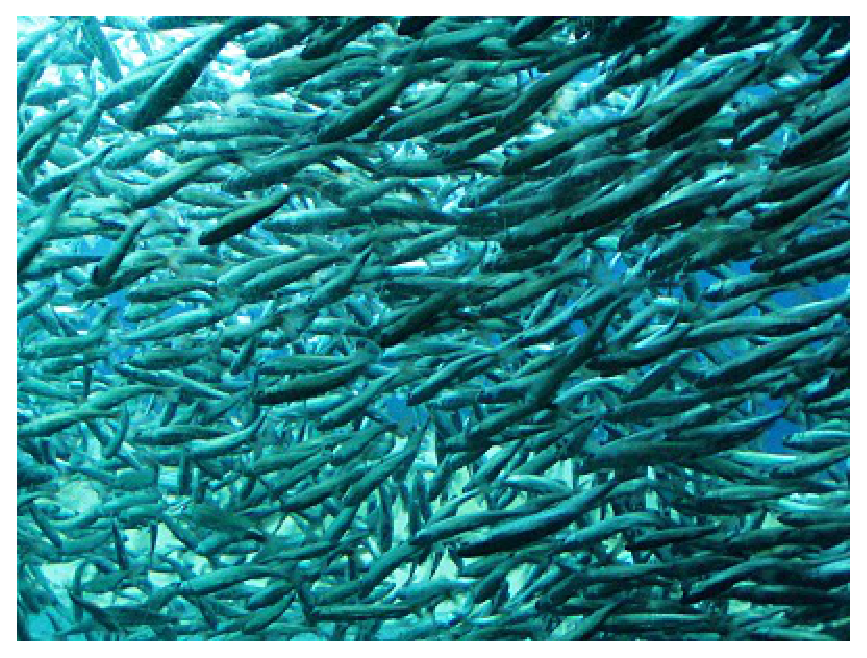
\includegraphics[height=1.60in]{fishes.eps}
\end{figure}

\end{frame}

\begin{frame}\frametitle{Learning from High-Dimensional Streaming Data}

We want to grab structures, patterns and rules from high-dimensional, rapid data streams.

\begin{figure}
\centering

\includegraphics[height=1.70in]{bear.eps}
\end{figure}

\end{frame}

\begin{frame}\frametitle{Learning from High-Dimensional Streaming Data}

Challenges for current machine learning algorithms.

\begin{itemize}
\item Algorithms must operate with limited resources
\item Algorithms must produce models on real-time
\item Algorithms must cope with changes in data distribution
\end{itemize}

\pause

~

Alternate approach: \alert{Demand-Driven Associative Classification}

\end{frame}

\begin{frame}\frametitle{Classification in High-Dimensional Streaming Data}

\begin{figure}
\centering
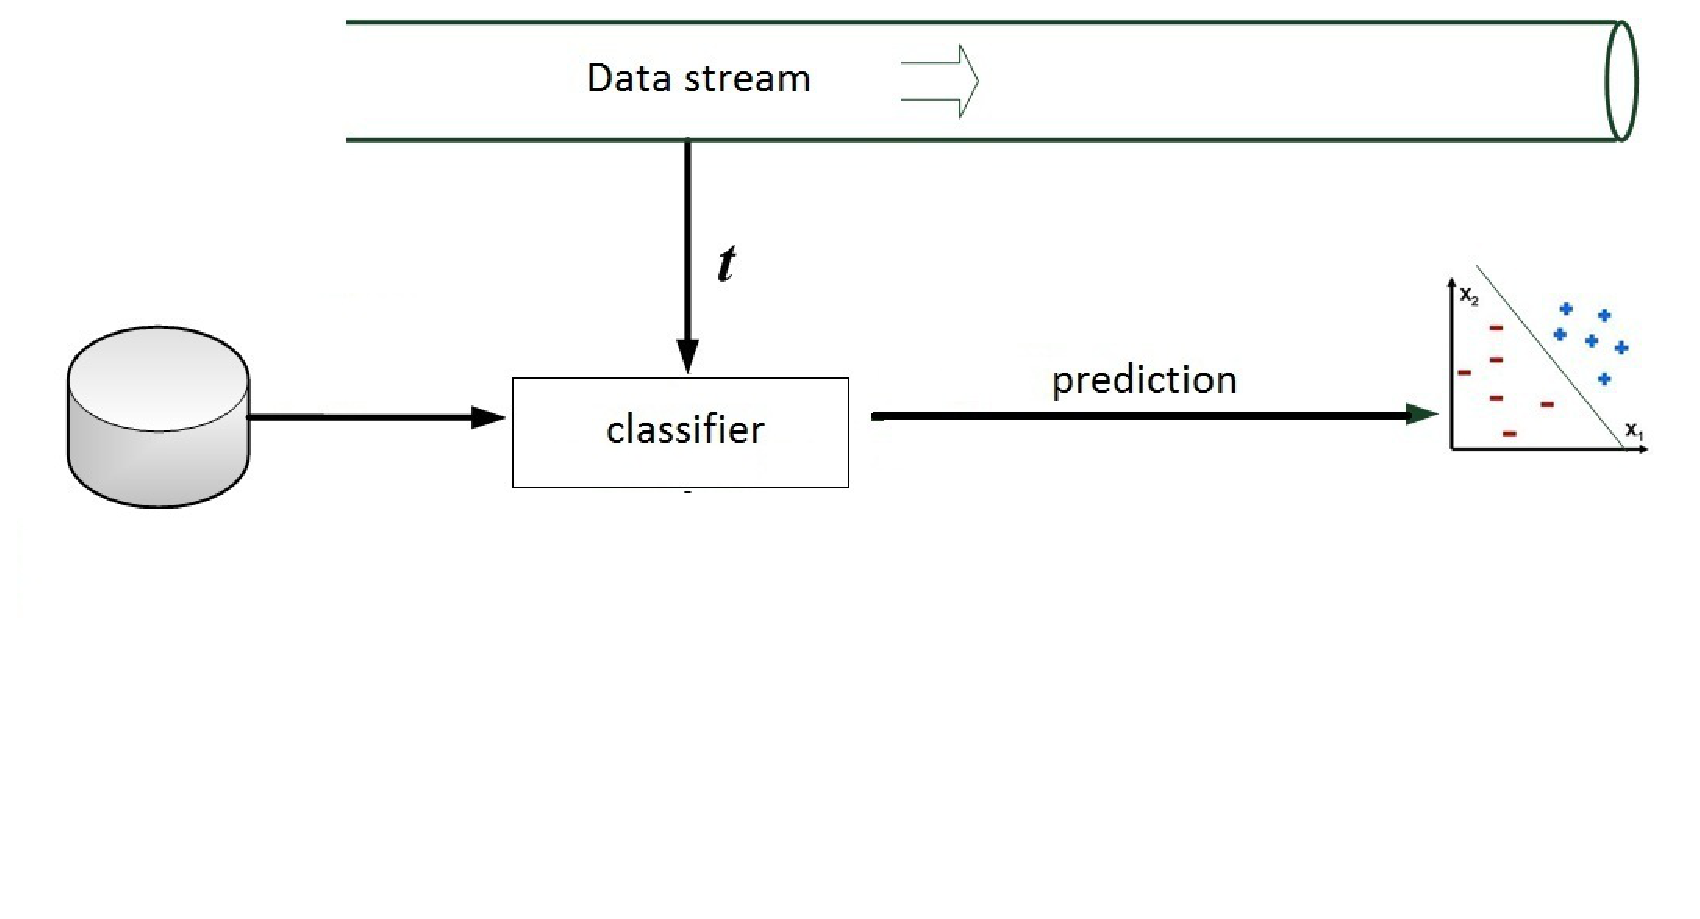
\includegraphics[height=1.80in]{stream2.eps}
\end{figure}

\end{frame}

\section{Associative Classification}
\begin{frame}\frametitle{Associative Classification}

Classifier is composed of a set of rules $\mathcal{X}\to c$.

\begin{itemize}
\item $\mathcal{X}$ is a feature-set
\item $c$ is the class variable
\end{itemize}

Rules are extracted from training (labeled) examples.

\begin{itemize}
\item Classifier is used in the test set
\item It outputs $\hat{p}(c|t)$ $\forall$ $t$: the likelihood of $c$ being the label for instance $t$
%\item $\sigma(\mathcal{X}\to c)$ is the number of times this rule occurs in the training data
%\item $\theta(\mathcal{X}\to c)$ is the accuracy of the rule
\end{itemize}

Advantage: Fast and smart algorithms for rule extraction.

\begin{itemize}
\item Effectiveness is competitive
\end{itemize}

\pause

Big problem: \alert{Exponential dependence on data dimension.}

\end{frame}

\begin{frame}\frametitle{Demand-Driven Associative Classification}

Wait for a test instance ($t$) to come.

\begin{itemize}
\item Extract only rules $\mathcal{X}\to c$ matching $t$ (i.e., $\mathcal{X}\subseteq t$)
\end{itemize}

Number of rules grows polynomially with data dimension ($n$).

\begin{itemize}
\item But it still grows exponentially with the size of $t$
\begin{itemize}
\item Fortunatelly, $O(2^{|t|})\ll O(n^{|t|})$
\end{itemize}
\end{itemize}

\end{frame}

\begin{frame}\frametitle{Contiguous Matching}

Test instance $t$ may be large (i.e., text).

\begin{itemize}
\item A pattern $\mathcal{X}=\{x_1, x_2, \ldots, x_k\}$ is contiguous if $\forall$ pair
$(x_i, x_{i+1})$,
$x_i$ is adjacent to $x_{i+1}$ in $t$.
\end{itemize}

The number of rules grows quadratically with the size of $t$ (i.e., enumeration via sliding window).

\begin{itemize} 
\item \alert{It grows linearly if we bound the cardinality of the rules}
\end{itemize} 

\end{frame}

\section{Applications}

\begin{frame}\frametitle{Protein Folding (PDB)}

Protein structure is related to its function.

\begin{itemize}
\item Predicts structure based on the amino acid sequence
\end{itemize}

\begin{figure}
\centering
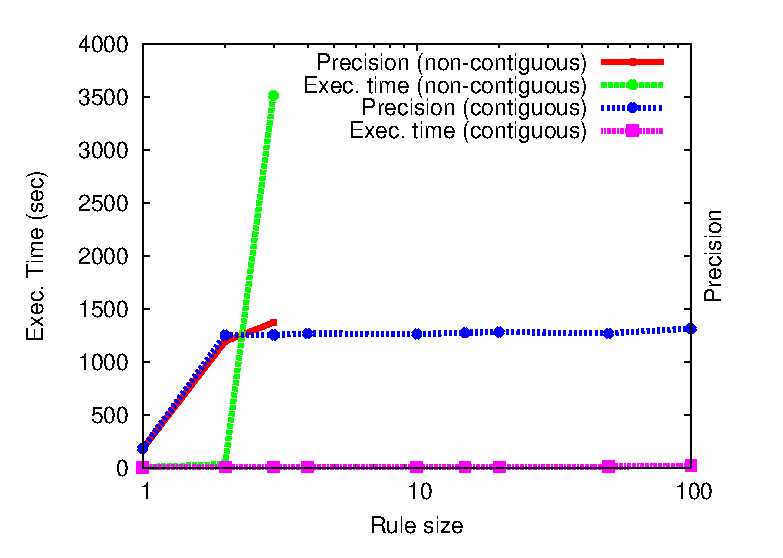
\includegraphics[height=1.40in]{tt.eps}
\end{figure}

%spire

\end{frame}

\begin{frame}\frametitle{Detecting Polluted Web Content (Youtube)}

Hard to obtain examples of spammers and promoters: Active Learning.

\begin{itemize}
\item Select examples that demand the least number of rules
\item Select most hard examples
\end{itemize}

\begin{figure}
\centering
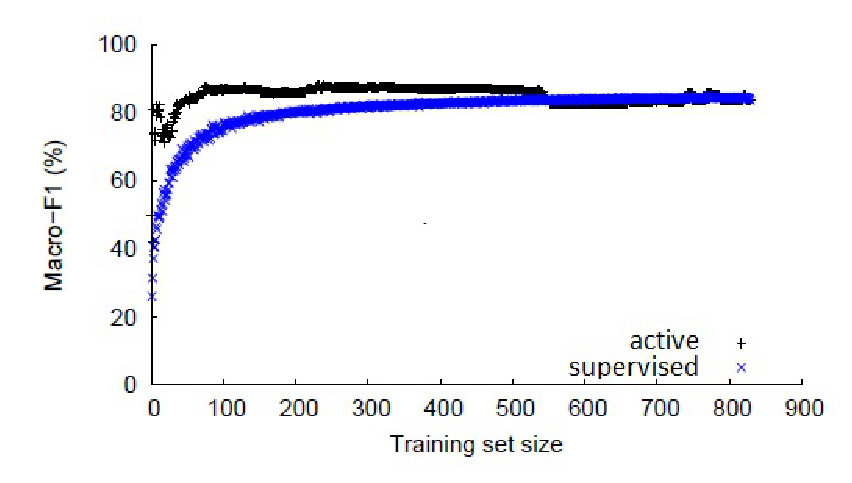
\includegraphics[height=1.40in]{active.eps}
\end{figure}

%tsmc

\end{frame}

\begin{frame}\frametitle{Multi-Objective Recommender Systems (Movielens)}

Selective Sampling and Aggregation.

\begin{itemize}
\item Select examples with most divesified, accurate or novel items.
\item Aggregate results based on Pareto optimality
\end{itemize}

%pkdd

\begin{figure}
\centering
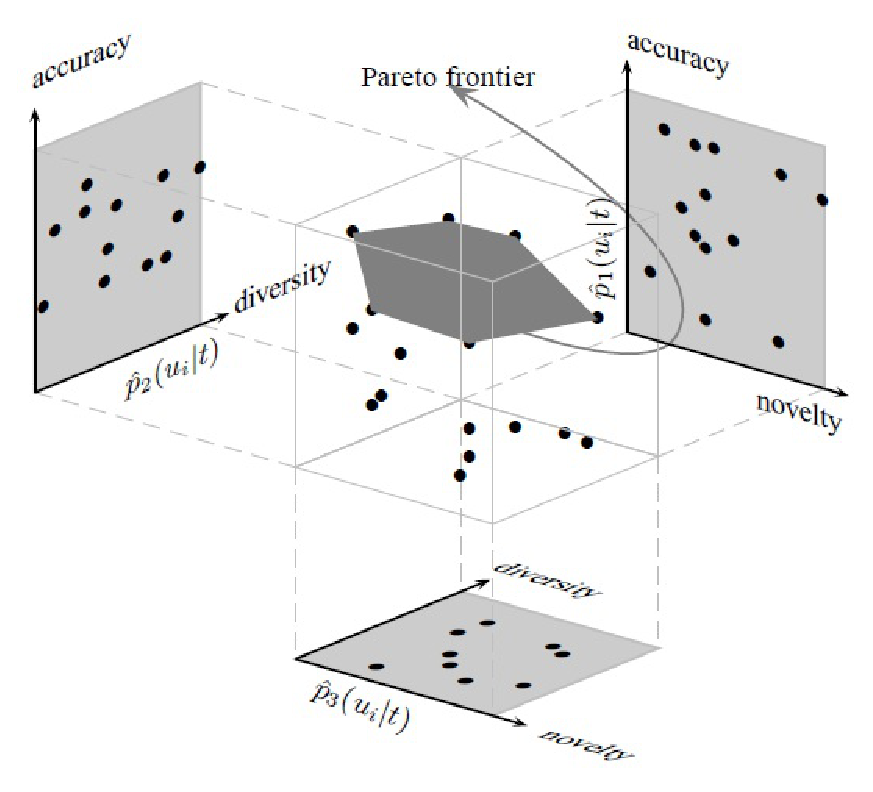
\includegraphics[height=1.90in]{front.eps}
\end{figure}

\end{frame}

\begin{frame}\frametitle{Sentiment Analysis}

Self-Training and Concept Drift

\begin{figure}
\centering
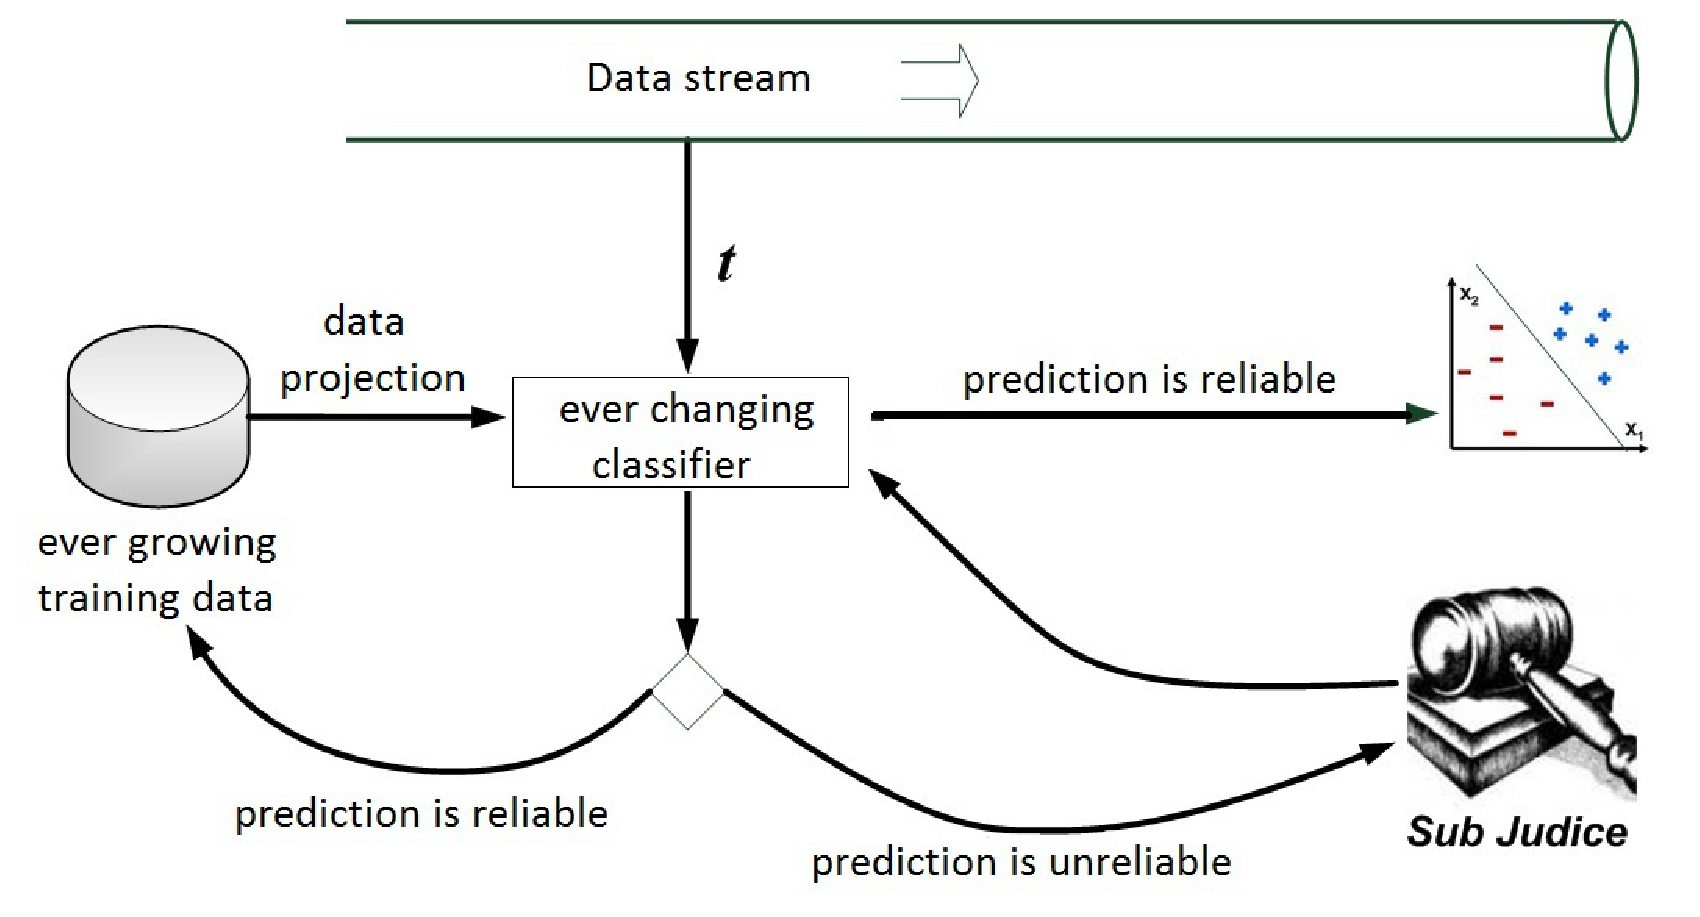
\includegraphics[height=1.80in]{stream.eps}
\end{figure}

\begin{itemize}
\item 
The only and all the rules that must be updated due to the inclusion of a labeled example $<t, c>$ are those matching $t$.
\end{itemize}

\end{frame}

\begin{frame}\frametitle{Sentiment Analysis}

Keeping the classifier always up-to-date as data is updated is challenging.

\begin{itemize}
\item 
The only and all the rules that must be updated due to the inclusion of a labeled example $<t, c>$ are those matching $t$.
\end{itemize}

\alert{The classifier is totally incremental.}

\begin{itemize}
\item Highly practical
\end{itemize}

\end{frame}


\begin{frame}\frametitle{Sentiment Analysis (Twitter) - SIGIR 11}

\vspace{-0.1in}
\begin{figure}
\centering
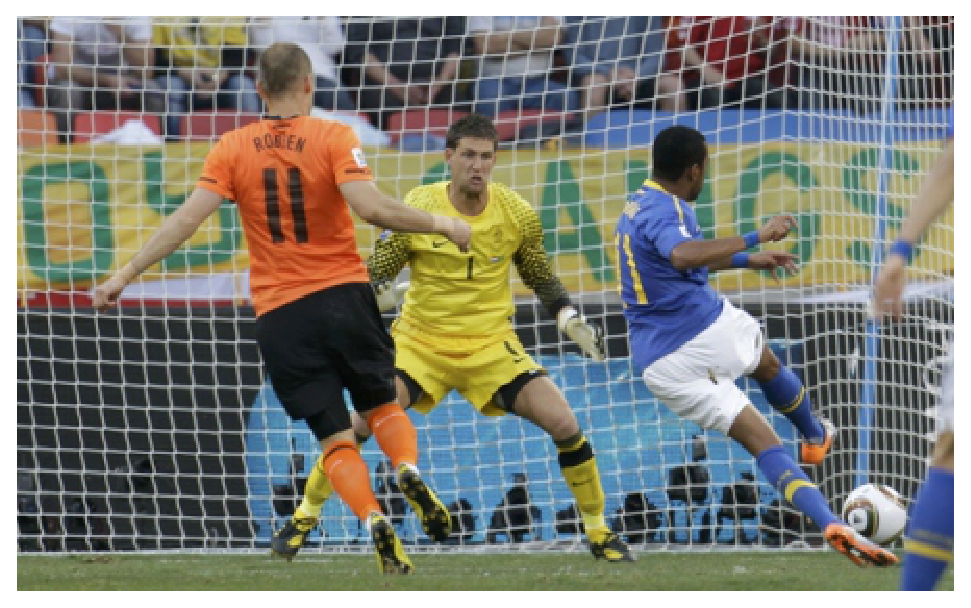
\includegraphics[height=1.00in]{golrobinho.eps}
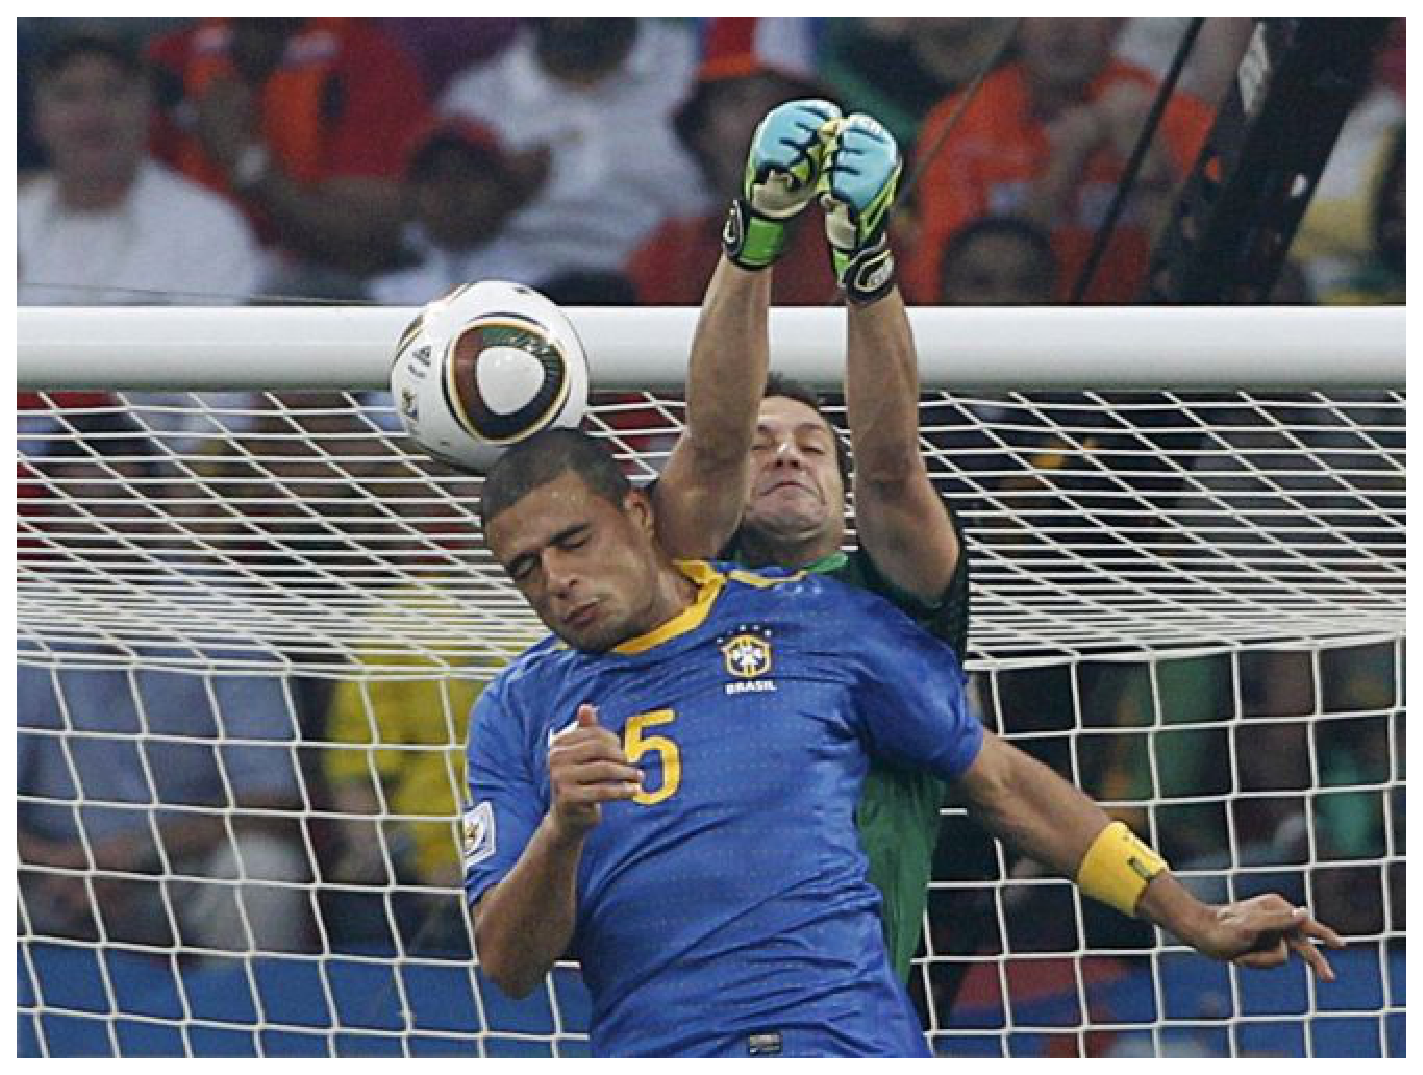
\includegraphics[height=1.00in]{contra.eps}
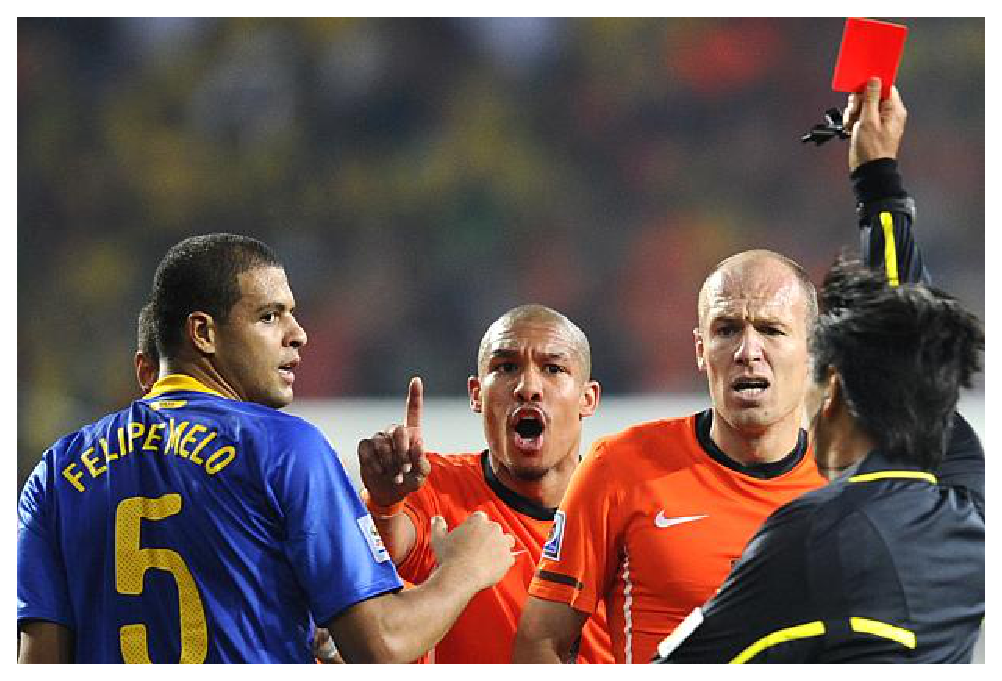
\includegraphics[height=1.00in]{vermelho.eps}
\end{figure}

\pause

\vspace{-0.15in}
\begin{figure}
\centering
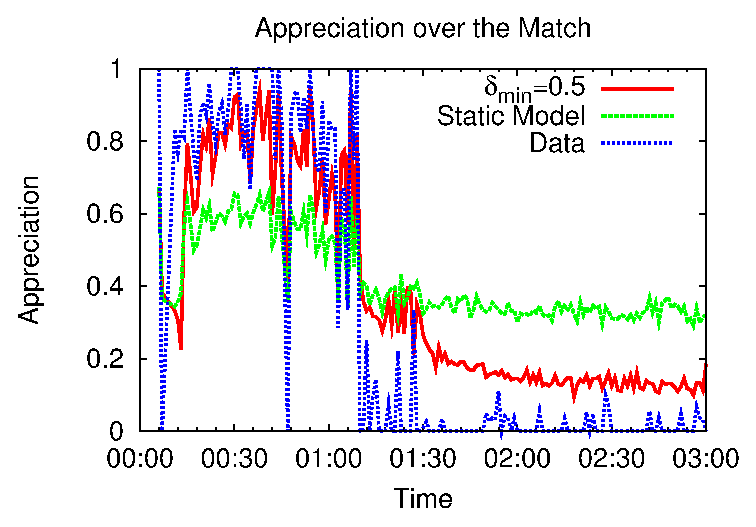
\includegraphics[height=1.40in]{fmpos.eps}
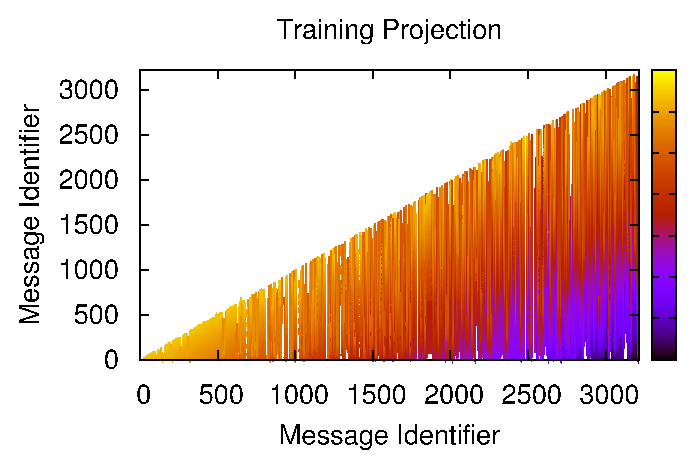
\includegraphics[height=1.40in]{fmloc.eps}
\end{figure}

\end{frame}

\begin{frame}\frametitle{Sentiment Analysis (Twitter) - SIGIR 11}

\vspace{-0.1in}
\begin{figure}
\centering
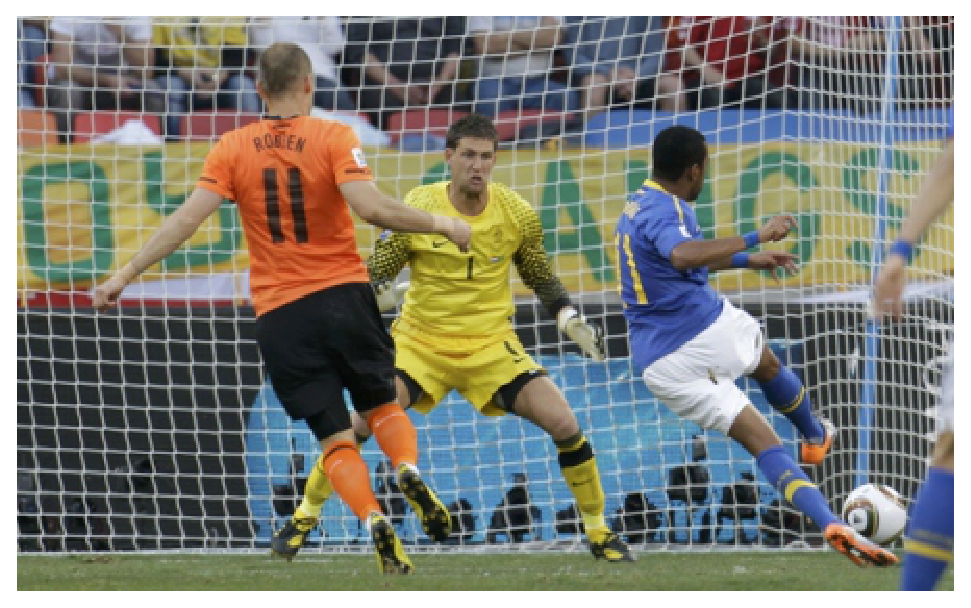
\includegraphics[height=1.00in]{golrobinho.eps}
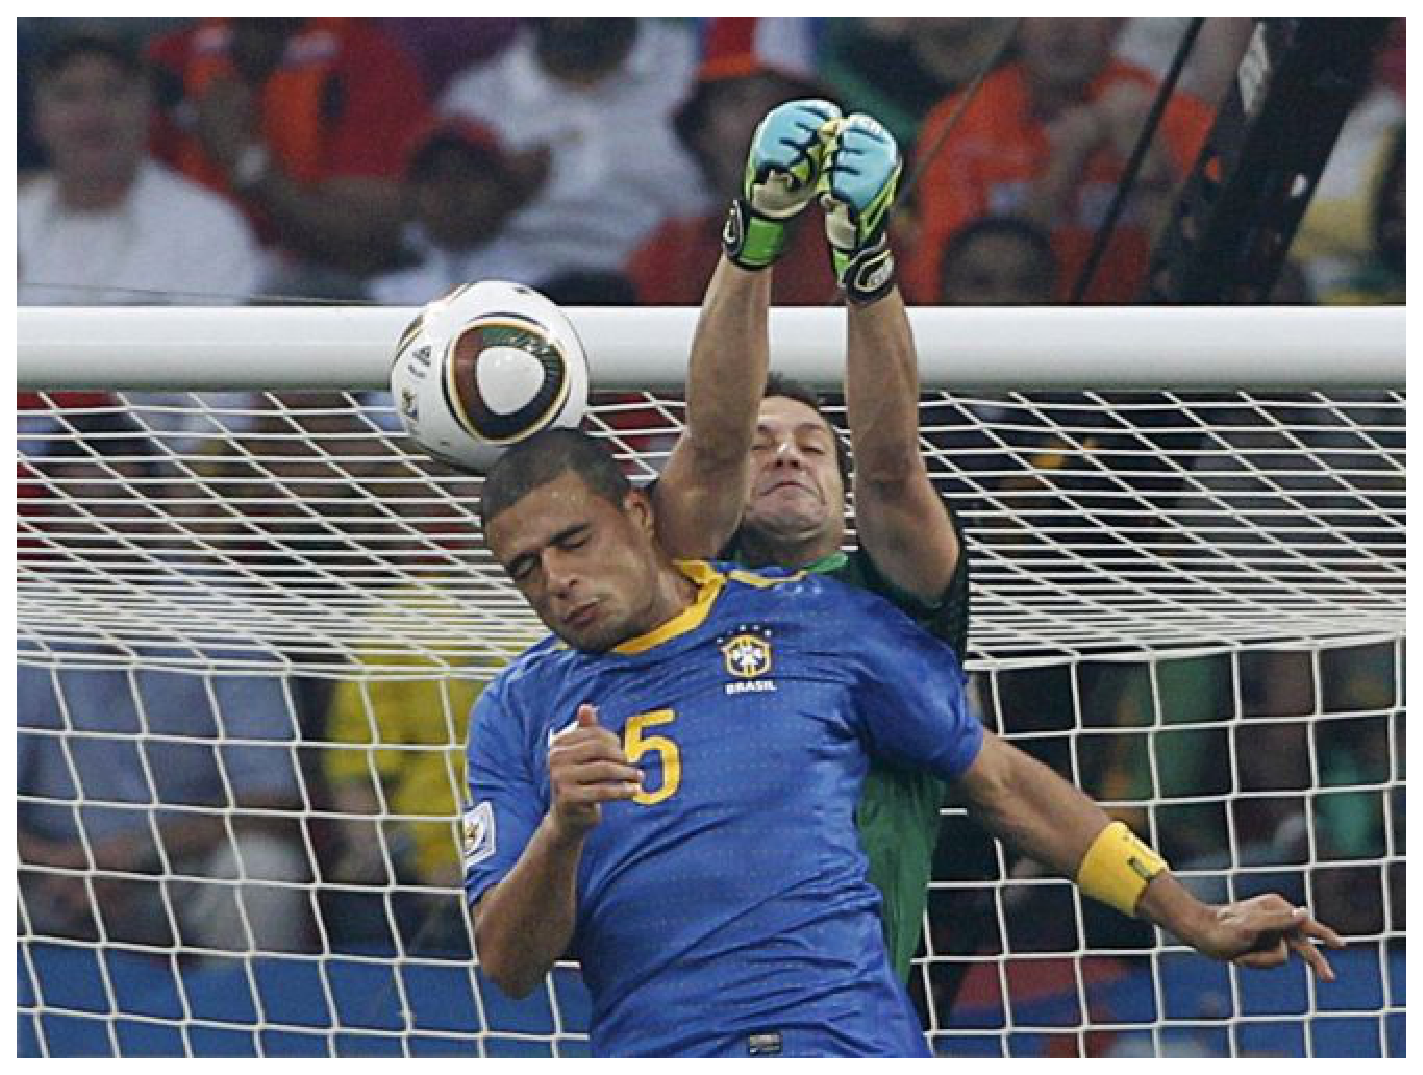
\includegraphics[height=1.00in]{contra.eps}
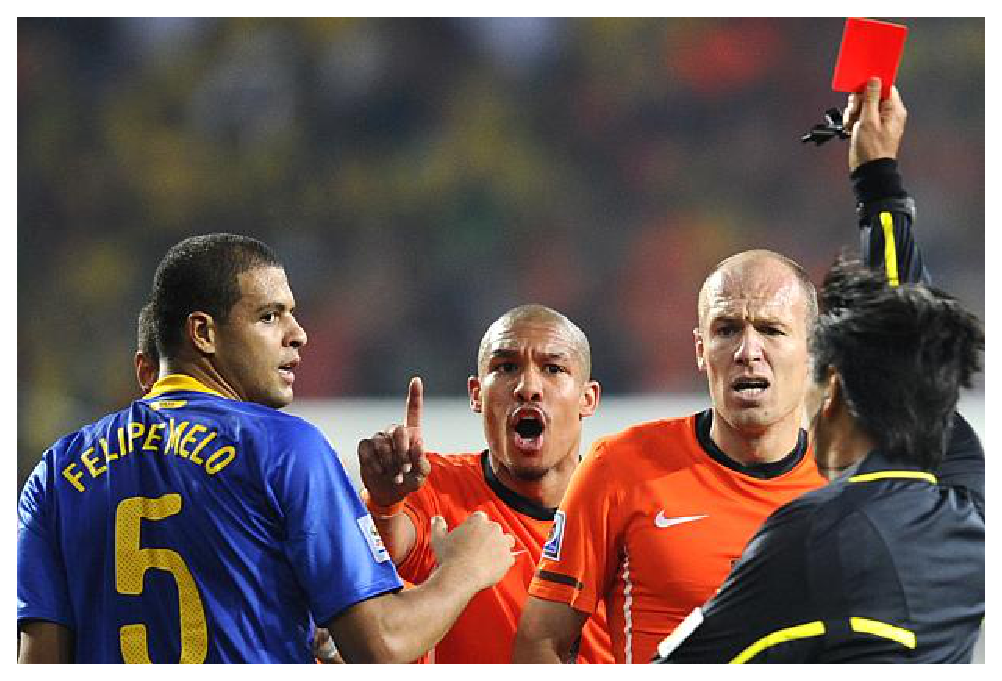
\includegraphics[height=1.00in]{vermelho.eps}
\end{figure}

\vspace{-0.15in}
\begin{figure}
\centering
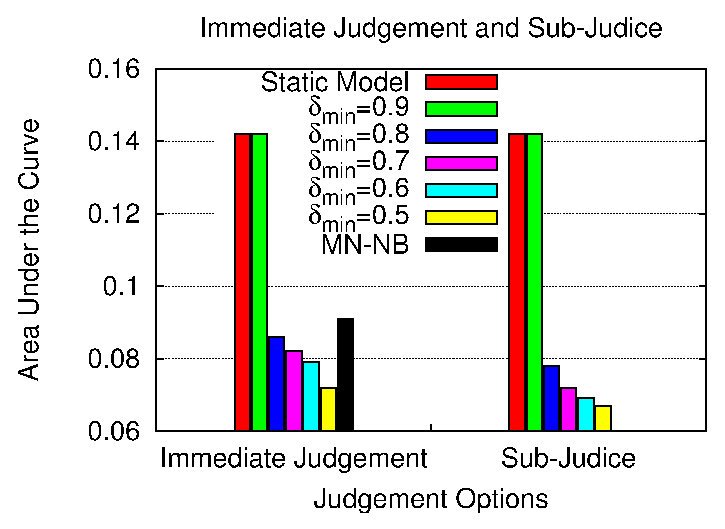
\includegraphics[height=1.40in]{fmarea.eps}
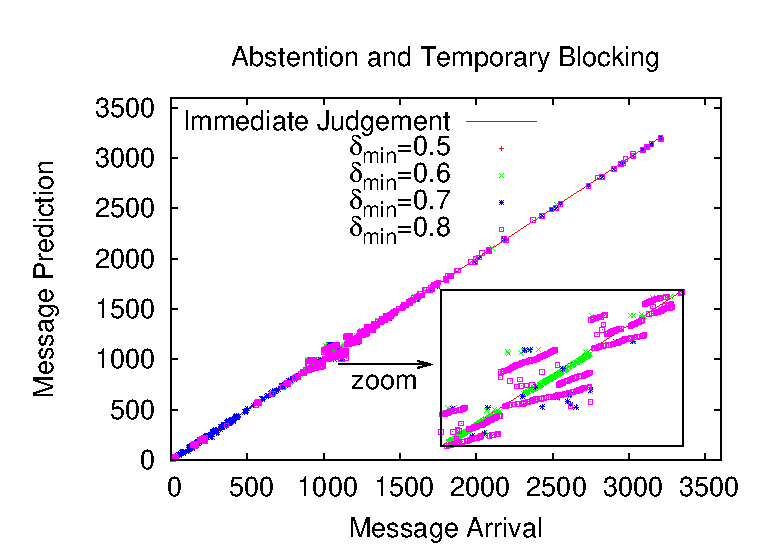
\includegraphics[height=1.40in]{fmmom.eps}
\end{figure}

%websci
%sigir11

\end{frame}

\begin{frame}\frametitle{Sentiment Analysis (Twitter) - WEBSCI 11}

\begin{figure}
\centering
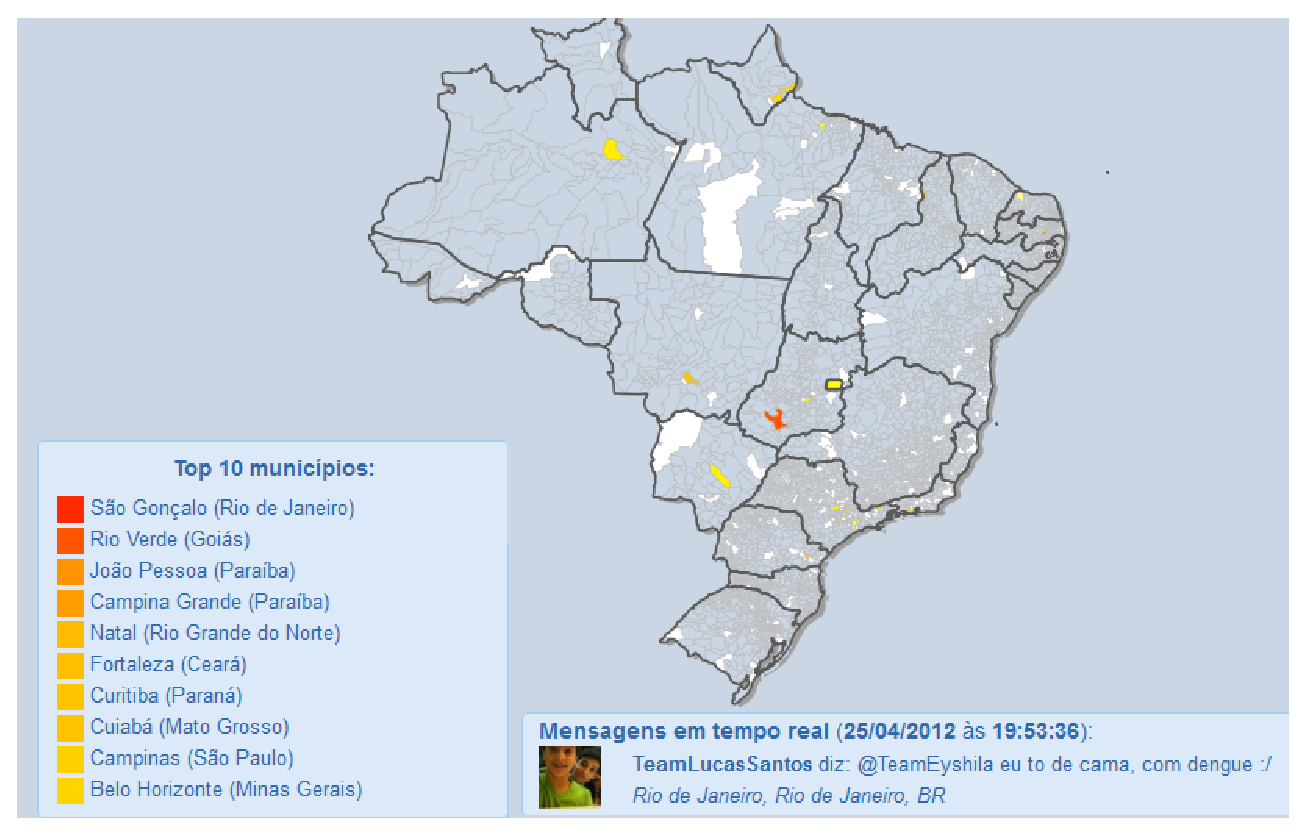
\includegraphics[height=2.50in]{dengue.eps}
\end{figure}

\end{frame}

\begin{frame}\frametitle{Named Entity Disambiguation (Twitter) - ACL 12}

Given a stream of messages and a list of
names $n_1, n_2, . . . , n_k$ used for mentioning a specific entity $e$.

\begin{itemize}
\item We must monitor the stream
and predict whether an incoming message containing
$n_i$ indeed refers to $e$ (positive example) or not
(negative example).
\end{itemize}

\begin{figure}
\centering
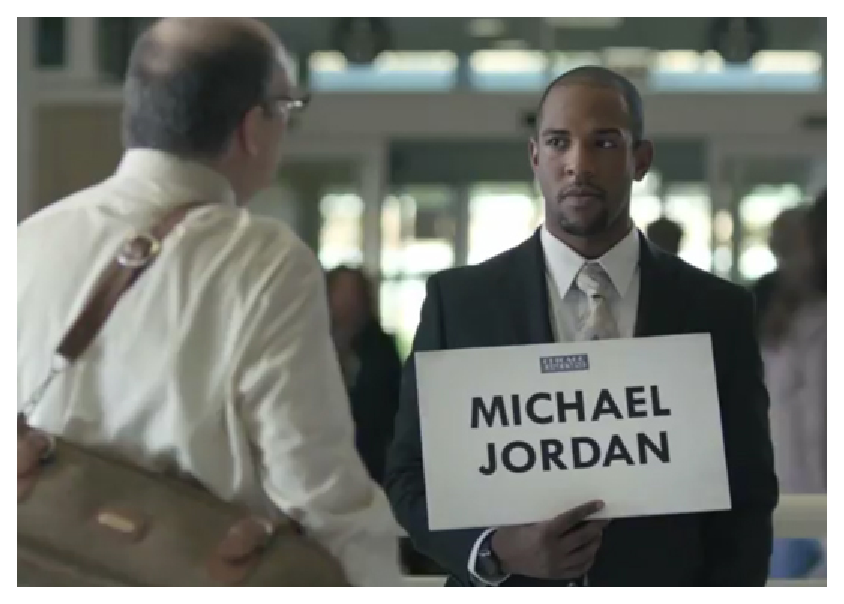
\includegraphics[height=1.40in]{mj.eps}
\end{figure}

\end{frame}

\begin{frame}\frametitle{Named Entity Disambiguation (Twitter) - ACL 12}

Expectation-Maximization: positive examples plus unlabeled data.

\begin{itemize}
\item Initially, unlabeled examples are treated as negative ones. The process iterates changing labels (i.e., $x^{\varominus\to\varoplus}$) until convergence.
\begin{itemize}
\item Label changing operation for instance $t$ is triggered if $\hat{p}(\varoplus, t)$ is greater than a threshold. Each instance may have a different threshold.
\end{itemize}
\end{itemize}

%\begin{figure}
%\centering
%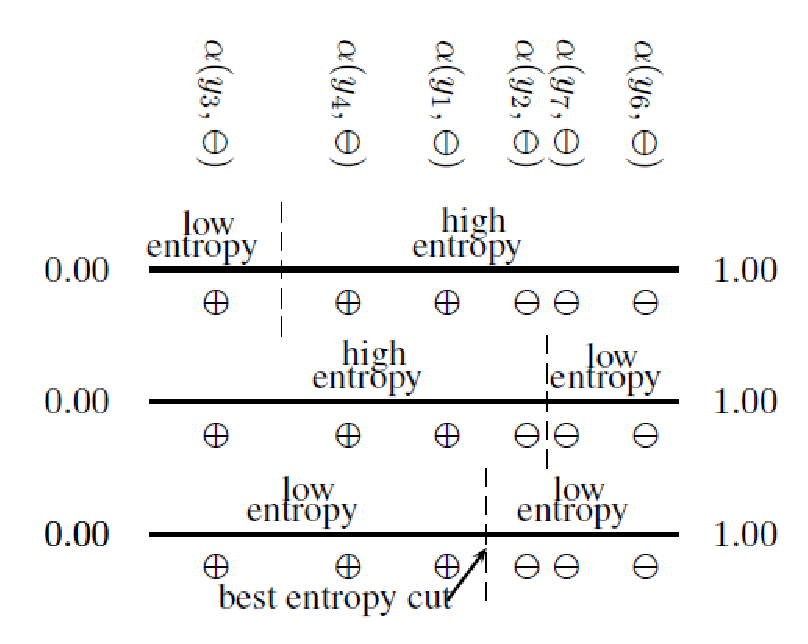
\includegraphics[height=1.40in]{em.eps}
%\end{figure}

Operation $x^{\varominus\to\varoplus}$ changes the data.

\begin{itemize}
\item 
All rules that must be updated
due to operation $x^{\varominus\to\varoplus}$ are those matching instance $x$
\end{itemize}

\alert{The classifier is totally incremental.}

\end{frame}

\begin{frame}\frametitle{Named Entity Disambiguation (Twitter) - ACL 12}

\begin{figure}
\centering
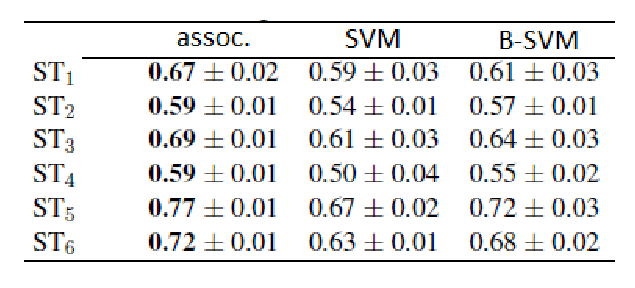
\includegraphics[height=1.00in]{disam.eps}
\end{figure}

\end{frame}

\section{Thank you}
\begin{frame}{Thank You!}
\begin{center}
\tt adrianov@dcc.ufmg.br\\
%\animategraphics[height=2.8in,autoplay,controls]{12}{em_}{0}{28}
%\animategraphics[autoplay,loop,height=5cm]{1}{em2_}{0}{28} 
\end{center}
\end{frame}

\end{document}
